\Chapter{REVUE DE LITTÉRATURE}\label{sec:RevLitt}
Cette section aura pour but de dresser l'état des connaissances sur les politiques de stationnement, l'estimation de la capacité de stationnement, les outils d'analyse d'images satellites utilisés pour la détection automatique d'objets, les coûts associés à la provision du stationnement et les méthodes d'estimation basées sur des données géospatiales.

\section{Typologie de stationnement}\label{sec:typologie_stationnement}
  \textcite{morency_stationnement_2017} détaillent des typologies de stationnement hors rue et sur rue pour la région métropolitaine de Montréal. Elles sont montrées aux figures \ref{fig:Typo_Stat_hors_rue} et \ref{fig:Typo_Stat_sur_rue}
  \begin{figure}[ht]
      \centering
      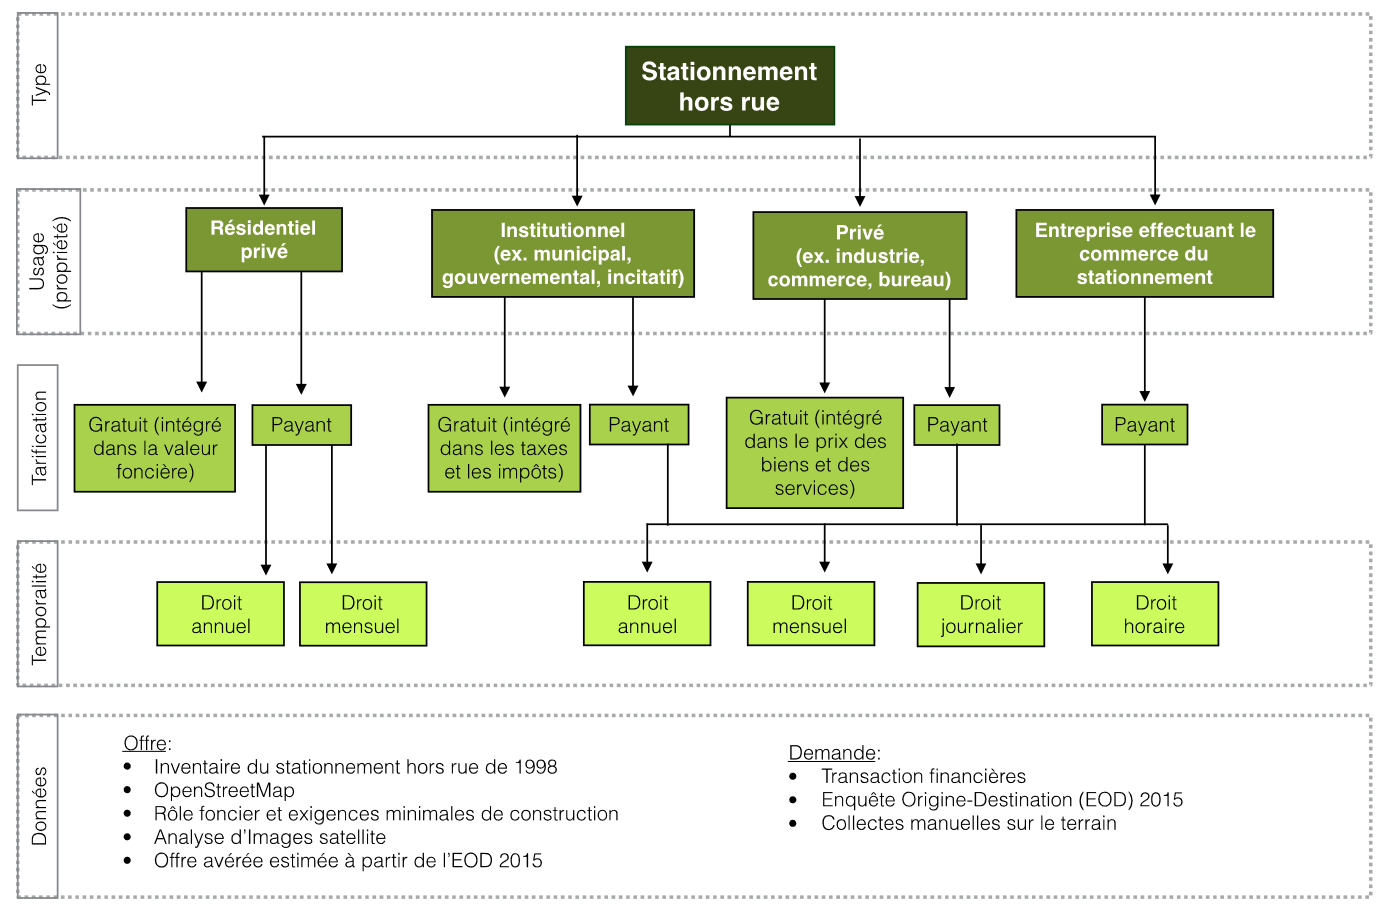
\includegraphics[width=1.0\textwidth]{dia/Typologie_Stationnement_hors_rue.png}
      \caption{Typologie de stationnement hors rue. Source: \cite{morency_stationnement_2017}}
      \label{fig:Typo_Stat_hors_rue}
  \end{figure}
  \begin{figure}[ht]
      \centering
      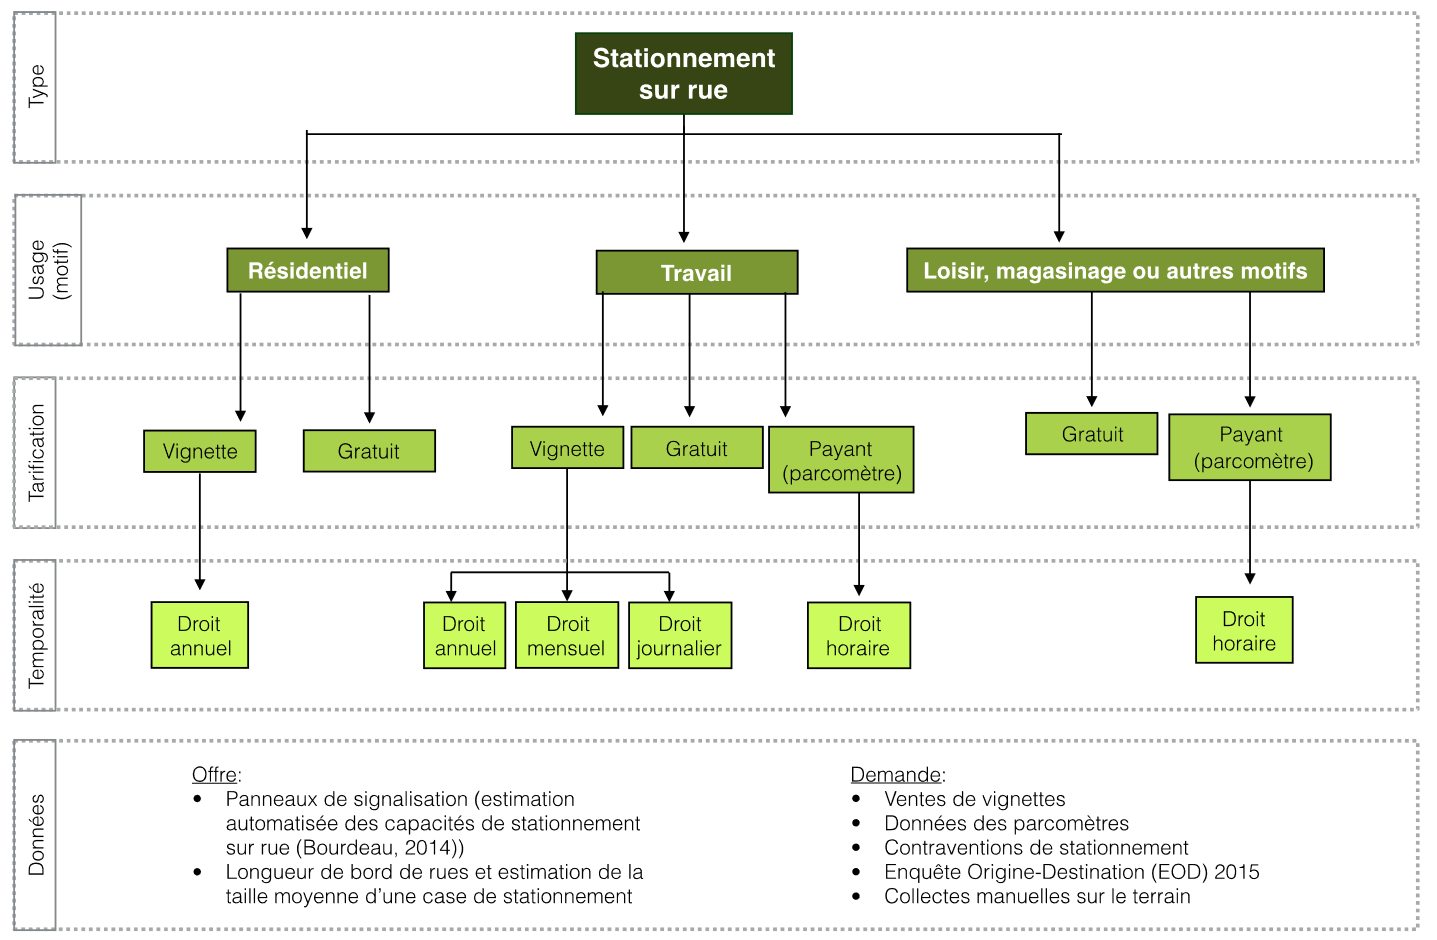
\includegraphics[width=1.0\textwidth]{dia/Typologie_Stationnement_sur_rue.png}
      \caption{Typologie de stationnement sur rue. Source: \cite{morency_stationnement_2017}}
      \label{fig:Typo_Stat_sur_rue}
  \end{figure}
  Il est important de noter qu'il n'existe pas, à la connaissance de l'auteur, un inventaire tel que celui complété par le ministère des Transports pour la ville de Montréal \parencite{consortium_cima_-_daniel_arbour_et_associes_inventaire_1998}. D'autre part, cet inventaire n'est pas mis à jour et n'est pas en accès libre.